\documentclass[12pt]{article}

\usepackage[style=phys,citestyle=authoryear,maxcitenames=2]{biblatex}
\addbibresource{stats-report.bib}

\usepackage[page]{appendix}

\usepackage{amsmath,amssymb,commath,mathabx,mathtools,physics,siunitx}
\usepackage{aas_macros}
\usepackage{float,subcaption}

\usepackage[margin=1in]{geometry}
\usepackage{setspace}
\doublespacing

%% Custom Units %%
\DeclareSIUnit{\parsec}{pc}
\DeclareSIUnit{\Msun}{M_\odot}
\DeclareSIUnit{\Lsun}{L_\odot}

\title{
Searching in the Dark
\\
Chasing Magnum Opus
}


\author{
  Jacob Lange, Chi Nguyen, Daniel Wysocki
}

\date{
  Statistical Methods for Astrophysical Sciences (ASTP-611)
  \\
  Spring 2016
}



\begin{document}

\maketitle


%%%%%%%%%%%%%%%%
% INTRO
% Everyone
%%%%%%%%%%%%%%%%
\section{Introduction}
\label{sec:intro}
The detection of gravitational waves (GW) in Feburary(ref) opened a new era of astronomy; however, it is only in sync with electromagnetic astronomy that the most physics can be discovered. Electromagnetic counterparts are expected from binary sources involving matter i.e. neutron star-neutron star and neutron star-black hole. Because of this, GW detectors will work in conjunction with electromagnetic telescopes to observe a GW source. Some of these will yield weak, nearly isotropic electromagnetic counterparts and others will not. GW detectors will identify sources characterized by its chirp mass:

\begin{equation}
\label{chirp_mass}
M_{c}=\frac{(m_{1}m_{2})^{3/5}}{(m_{1}+m_{2})}
\end{equation}

Figure \ref{fig:chirp} is the full data set in terms of chirp mass. The electromagnetic counterparts events are seperated from the other events by color. This report is organized as follows. Section \ref{sec:dist} describes the developement of the chirp mass distribution, Section \ref{sec:classifier} descibes a electromagnetic followup classifier based on the data, and Section 4 will state our conclusions.
\begin{figure}
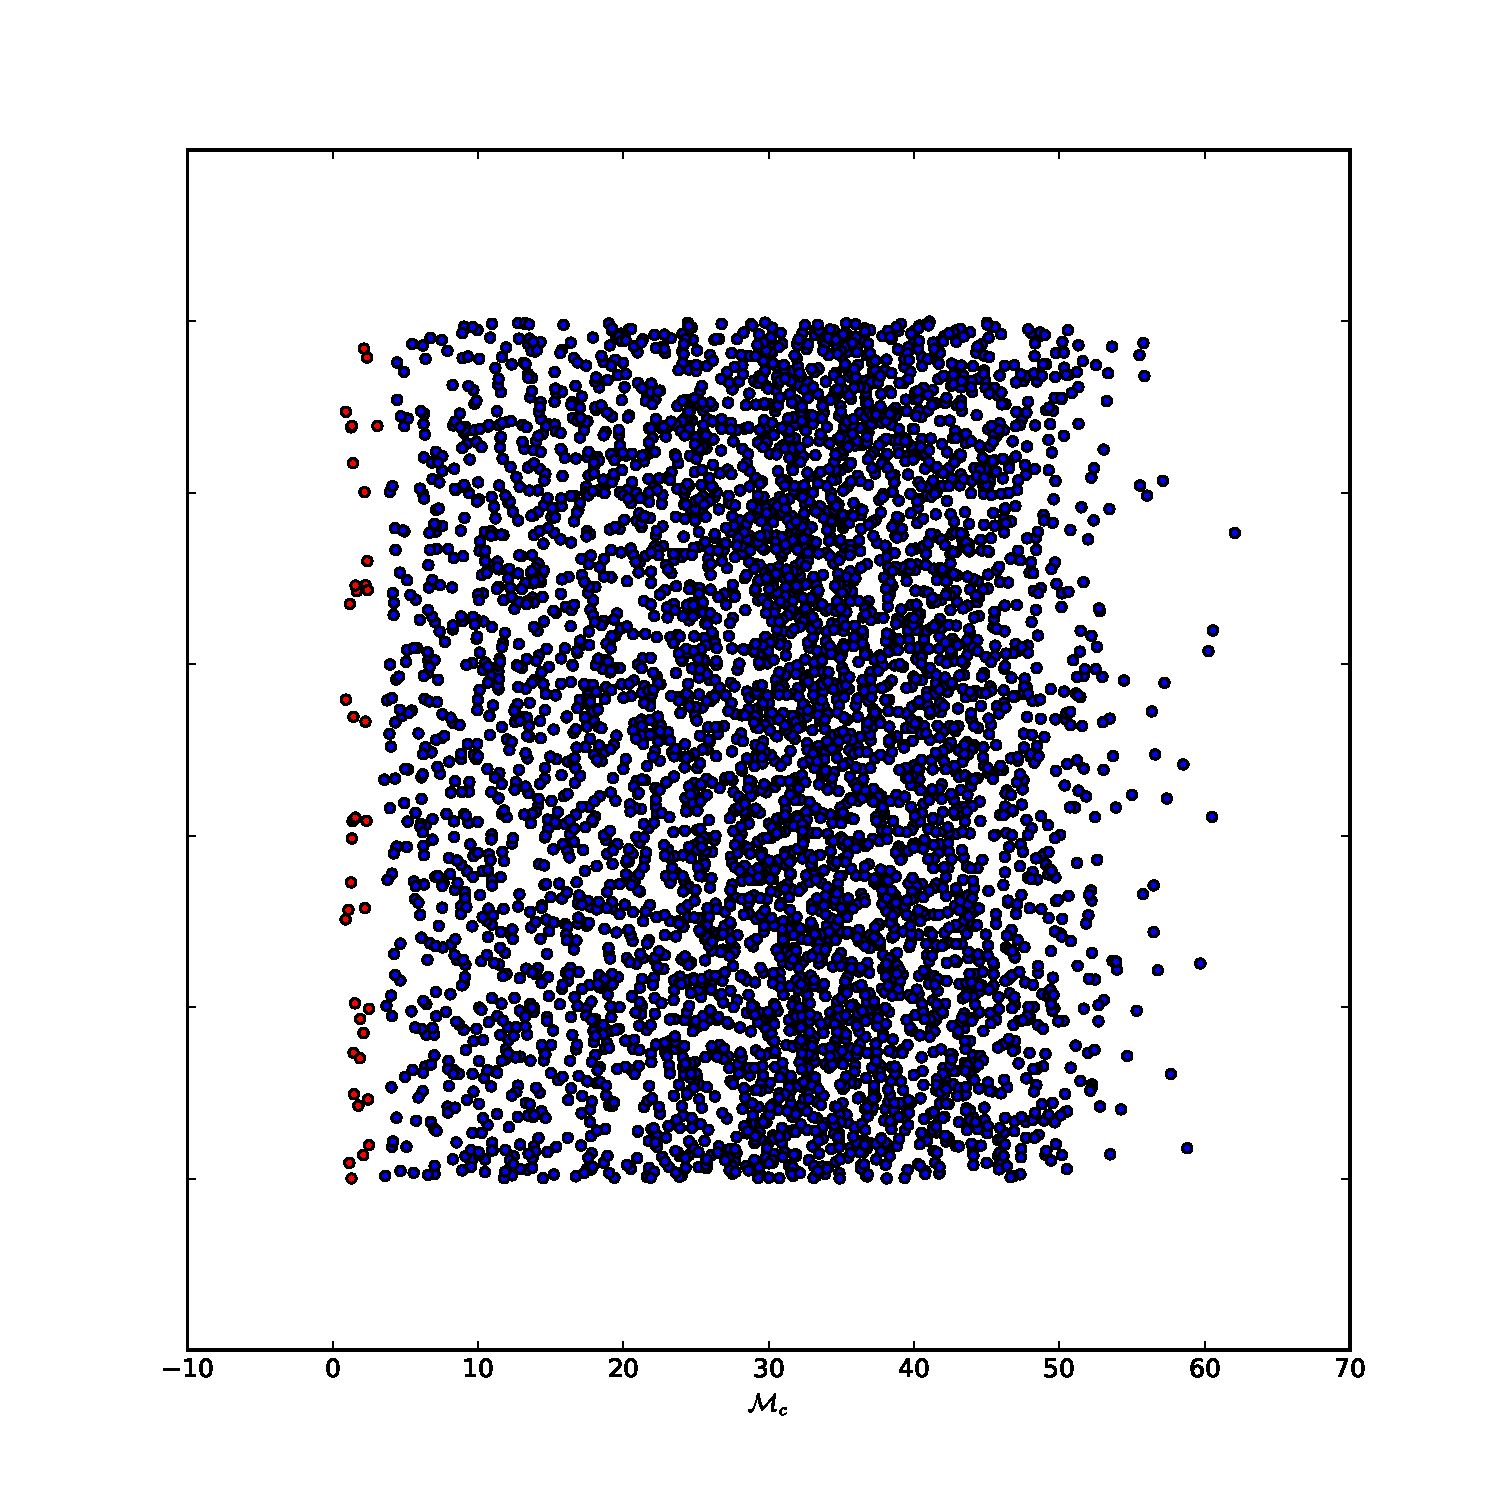
\includegraphics[width=\columnwidth]{output/jake/chirp-mass-classes.pdf}
\caption{This figure shows all the 5000 events' chirp mass. Here the y-axis is a uniform random number between zero and one. The events that have an electromagnetic counterpart are in red, and the events without a electromagnetic counterpart are in blue.}
\label{fig:chirp}
\end{figure}
See Section \ref{sec:discussion} and Appendix \ref{app:example}. Example text citation is \textcite{2012ApJ...759...52D}, or in parenthesis with a page number \parencite[pg 2]{2012ApJ...759...52D}.


%%%%%%%%%%%%%%%%
% QUESTION 1
% Dan & Chi
%%%%%%%%%%%%%%%%
\section{Chirp Mass Distribution}
\label{sec:dist}

\subsection{Density Estimation}
\label{sec:density}

We use a histogram to estimate the merger rate as a function of $\mathcal{M}_c$, using Knuth's rule to determine the bin size (See Figure \ref{fig:chirp}). Since we are interested in the intrinsic rate, not just that of detected events, we weigh each point by the inverse of the spacetime volume in which we are sensitive to it, $w = 1 / VT$. Binaries with a higher chirp mass are easier to detect, so we do not want to count them as heavily. For a given chirp mass, we are sensitive out to a distance
%
\begin{equation}
  D(\mathcal{M}_c) =
  \SI{200}{\mega\parsec} \qty( \mathcal{M}_c / \SI{1.2}{\Msun} )^{5/6}
\end{equation}
%
which corresponds to a volume
%
\begin{equation}
  V(\mathcal{M}_c) = \frac{4}{3} \pi D^3(\mathcal{M}_c).
\end{equation}
%
Multiplying this by the time spent observing, $T = \SI{0.6}{yr}$, gives us the spacetime volume $V(\mathcal{M}_c) T$.

To obtain uncertainties in our histogram, we take the square root of the sum-of-squares of the weights within that bin, i.e.
%
\begin{equation}
  \sigma_k = \sqrt{\sum_i w_i^2},
\end{equation}
%
which was taken from \textcite{weighted-hist}. This reduces to $\sqrt{N}$ in the case of an unweighted histogram, as $w_i = 1$, so $\sum_i w_i^2 = N$.

We also over-plot a pure power law. To do this, we employ Bayesian linear regression, fitting a straight line to $\log r$ versus $\log \mathcal{M}_c$, and transforming back to linear space. This is also shown in Figure \ref{fig:chirp}.

\begin{figure*}[ht]
  \centering
  \begin{subfigure}[c]{\textwidth}
    \centering
    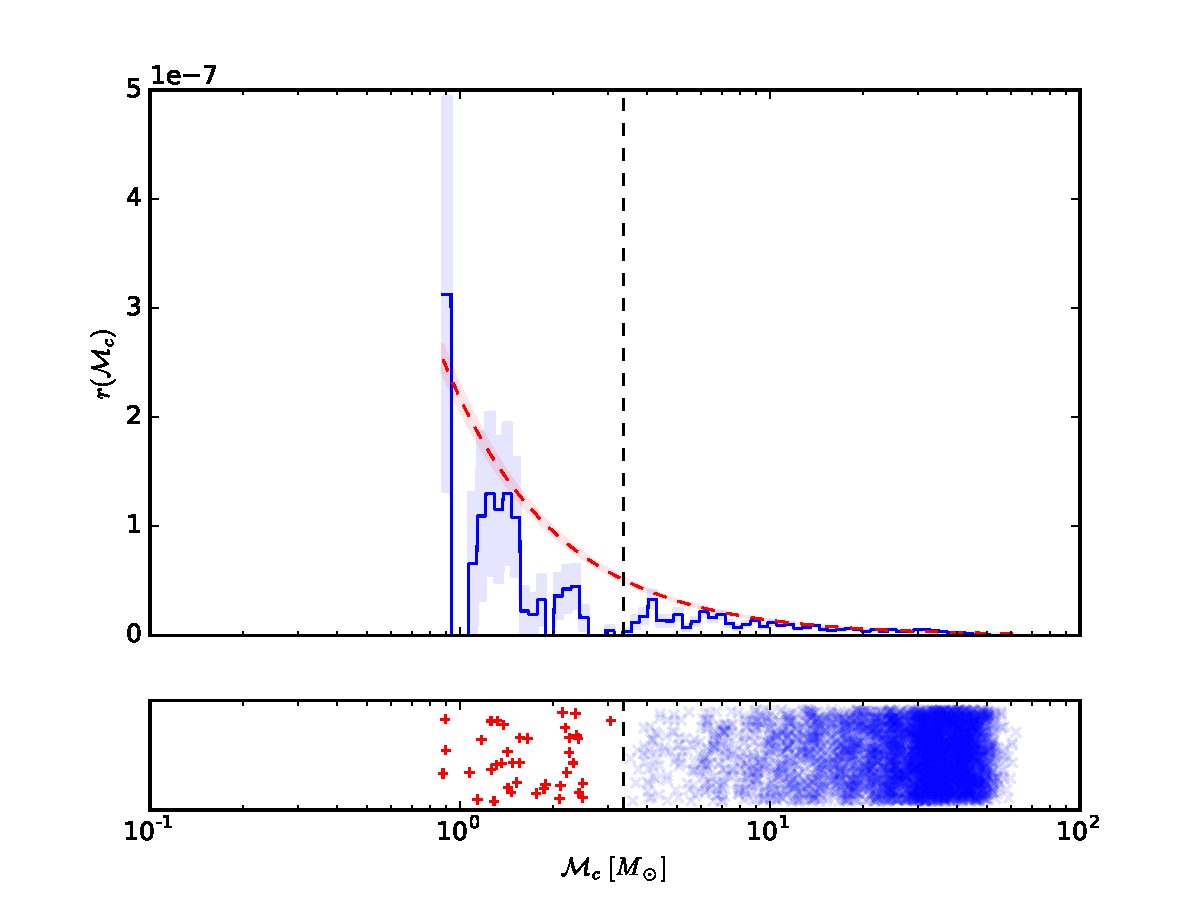
\includegraphics[height=0.4\textheight]{img/chirp-mass-distribution}
    \caption{}
    \label{fig:chirp-linear}
  \end{subfigure}

  \begin{subfigure}[c]{\textwidth}
    \centering
    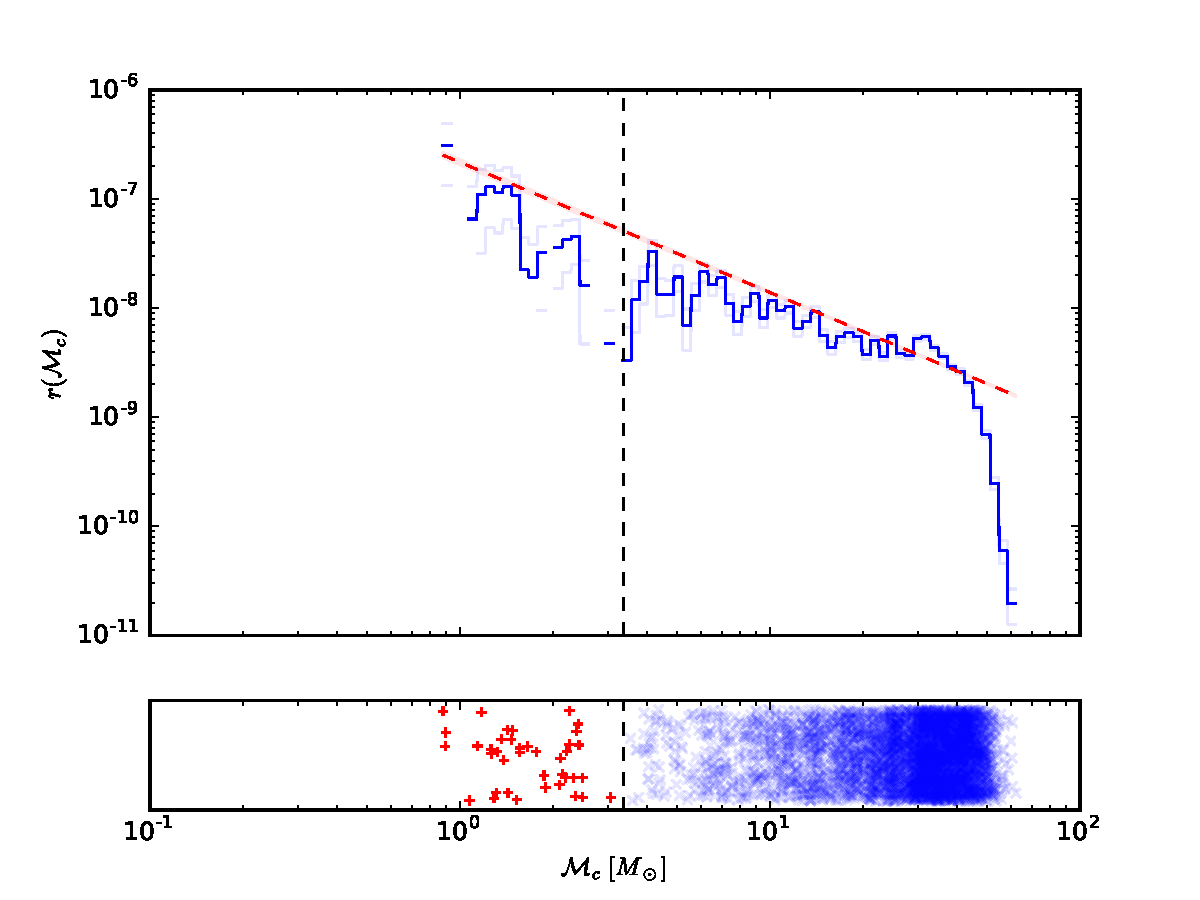
\includegraphics[height=0.4\textheight]{img/chirp-mass-log-distribution}
    \caption{}
    \label{fig:chirp-log}
  \end{subfigure}

  \caption{Estimated rate of compact binary mergers, based on 5000 synthetic observations. Rate is shown in (\subref{fig:chirp-linear}) linear and (\subref{fig:chirp-log}) log scale. Blue line is weighted histogram fit. Red curve is power law fit. Shaded regions are 1-$\sigma$ error bars. Vertical dashed line is boundary between events with counterparts and without.}
  \label{fig:chirp}
\end{figure*} % Q1.1, Dan
\subsection{The Likelihood of Fitting Parameters}
\label{subsec:likelihood}

The likelihood estimator of each fitting parameter is:

\begin{equation}
\label{likelihood}
\ln{P(\{d\}|\lambda)} = \frac{-1}{2}\sum_{k} \qty{\frac{[r(x_k) -r_{\rm model}(x_k)]^2}{\sigma_r^2}}
\end{equation}

where $p_{\rm smooth}$ is the smoothing prior, defined to be:

\begin{equation}
\label{smoothing_prior}
p_{\rm smooth} = \exp{-\int \qty[\dv[n]{(r)}{(x)}]^2 \dd{x}}
\end{equation}

In theory, $p_{\rm smooth}$ can be any $n^{\rm th}$ derivative. To make our code robust, we define a function that takes n as an argument. The function then calls numpy.polynomial.polyder() to find the $n^{\rm th}$ derivative. Next, we square the $n^{\rm th}$ derivative and integrate it between the minimum and maximum of $x$. Here we choose $n = 3$. % Q1.2, Chi
\subsection{Model fitting}
\label{subsec:fitting}
We employed a Markov Chain Monte Carlo (MCMC) script to fit the coefficients of a polynomial model for $r(M_c)$. The MCMC uses the smoothing prior as defined in section \ref{subsec:likelihood}. We performed a least square fit first in order to obtain the initial guess for the coefficients of the model. % Q1.3, Chi



%%%%%%%%%%%%%%%%
% QUESTION 2
% Jake
%%%%%%%%%%%%%%%%

\section{Classifying GW Events that have Electromagnetic Countparts}
\label{sec:classifier}
\subsection{Overview}

\begin{figure}
  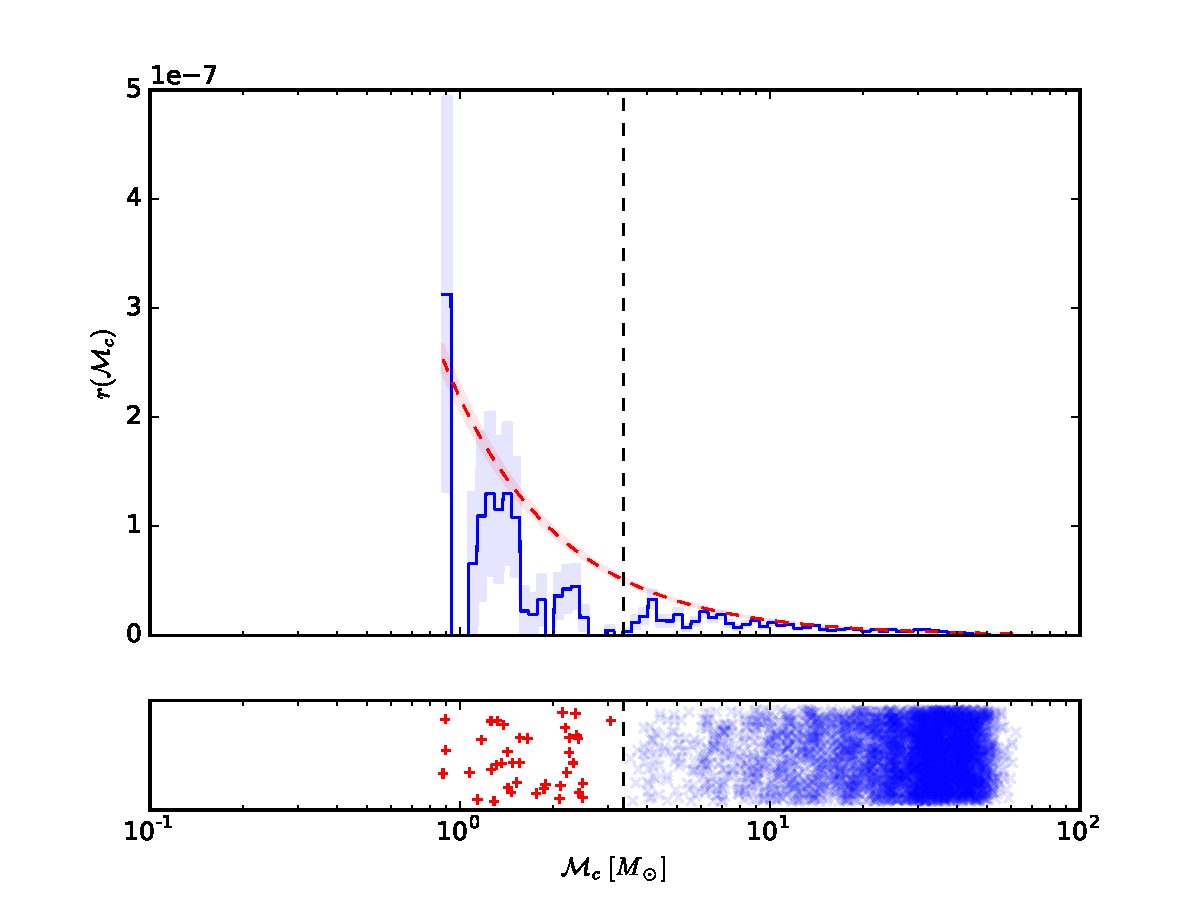
\includegraphics[width=\columnwidth]{img/chirp-mass-distribution}
  \caption{}
  \label{fig:chirp}
\end{figure}

\begin{figure}
  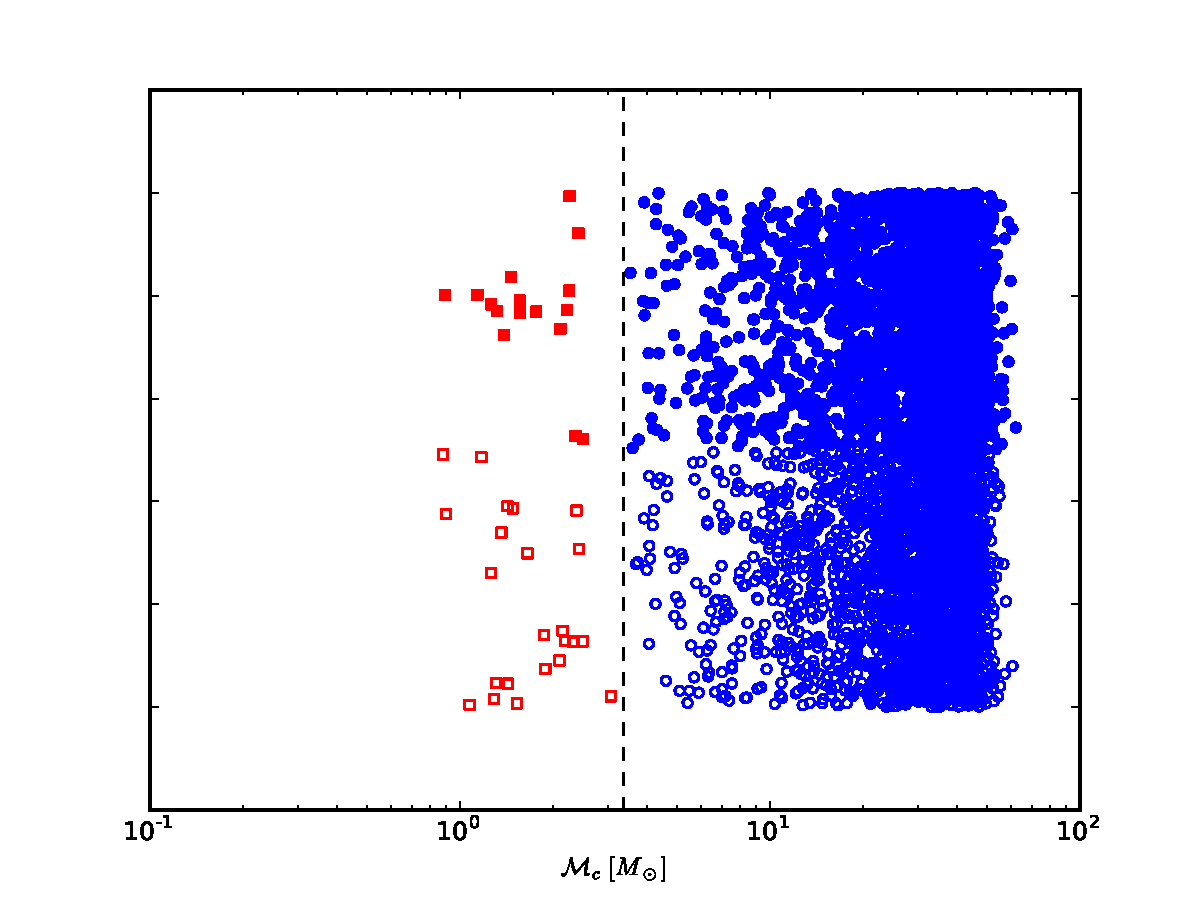
\includegraphics[width=\columnwidth]{img/classifier_comparison}
  \caption{This shows a selected set of the data. The red points represent the events with electromagnetic counterparts, and the blue points represent the events without electromagnetic counterparts. The filled points represent represent the train dataset, and the open points represent the rest of the data. The vertical line indicates the division between the two groups indicated by the classifier.}
  \label{fig:class}
\end{figure}

The GW observatory, the Laser Interferometer Gravitational Wave Observatory (LIGO), can provide very rapid mass estimates of candidate GW events. Since most of these detections are mostly binary black holes and electromagnetic followup is extremely expensive, only a few events can be followed up. We have therefore trained a classifier to determine if an event will have a electromagnetic followup. We trained this classifier on the first half of the data; we simply took the mid-way point betweewn the maximum chirp mass for the electromagnetic counterpart group and the nonelectromagnetic counterpart group. This can be seen in Figure \ref{fig:class}

\subsection{Method}
The classifier was constructed simply by taking the minimum chirp mass event of the other group (no electromagnetic counterparts) and the maximum chirp mass event of the electromagnetic counterpart group and finding the distance between those two events. This trained for the first half of the dataset. The result can be seen in Figure \ref{fig:half}; the vertical line represents half the distance between the maximum chirp mass of the electromagnetic counterpart group and the other group.

\subsection{Results}
The classifier correctly classified the two groups without any contamination. More importantly this was also the case when classifying the full data set. As you can see in Figure \ref{fig:all}, the classifier correctly classified the two groups without any contamination. In the Table \ref{tab:chirp} You can see the chirp mass for the maximum electromagnetic counterpart event and the minimum of the other group along with the chirp mass of the line that divides the group. This shows a clear distinction between the two group.



Figure \ref{fig:chirp} shows the rate vs the chirp mass with the dividing line from the classifier overplotted. This correlates to the two hump structure in the graph that represents the two groups (electromagnetic counterparts and others). Figure ... shows a similar correlation. The dividing clearly separates the two groups in  m$_{1}$-m$_{2}$ parameter space. % Jake


%\section{Conclusions}
%\label{sec:conclusions}
%We created a classifier to distinguish between GW events with and without electromagnetic counterparts. This classifier was trained using half of the data. The classifier correctly classified both groups completely without any contamination for both the training set and the full dataset. Figure ... and ... shows the correlation between 1D and 2D mass distributions and the classification of the two groups.










\end{document}